\documentclass[aspectratio=169,11pt]{beamer}
\usepackage[T1]{fontenc}
\usepackage[utf8]{inputenc}
\usepackage{lmodern,amsmath,amssymb,graphicx,tikz}
\usetikzlibrary{arrows.meta,calc}
\usetheme{default}
\usefonttheme{serif}
\setbeamercolor{normal text}{fg=black,bg=white}
\setbeamercolor{structure}{fg=black}
\setbeamercolor{frametitle}{fg=black}
\setbeamercolor{title}{fg=black}
\setbeamertemplate{navigation symbols}{}
\setbeamertemplate{footline}[frame number]
\setbeamertemplate{itemize items}[circle]
\setbeamersize{text margin left=8mm,text margin right=8mm}
\setlength{\parskip}{5pt}
\newcommand{\cO}{\mathcal O}
\newcommand{\cI}{\mathcal I}
\newcommand{\cA}{\mathcal A}
\newcommand{\db}{\bar\partial}
\newcommand{\C}{\mathbb C}
\newcommand{\Pj}{\mathbb P}
\newcommand{\norm}[1]{\lVert#1\rVert}
\newcommand{\src}[1]{\par\vfill{\scriptsize #1\par}}
\author{Daniel Gonz\'alez Casanova Azuela}

\title{Sections, embeddings, and weaker positivity}
\subtitle{Lecture 24 --- draft}
\date{Hodge theory}
\begin{document}
\begin{frame}\titlepage\end{frame}
\begin{frame}{Two applications, two choices of ideal}
Nadel gives
\[
H^q(X,K_X\otimes B\otimes\cI_h)=0\qquad(q>0)
\]
when \(i\Theta_h\ge\varepsilon\omega\).
\begin{enumerate}
\setlength{\itemsep}{10pt}
\item Choose singularities to prescribe values and derivatives of sections.
\item Choose singularities mild enough that \(\cI_h=\cO_X\).
\end{enumerate}
\end{frame}

\begin{frame}{Kodaira embedding theorem}
Let \(X\) be a compact complex manifold and \(L\) a holomorphic line bundle with a smooth metric of positive curvature.
\medskip
\par For all sufficiently large \(N\), global sections of \(L^N\) define a holomorphic embedding
\[
\boxed{\Phi_N:X\hookrightarrow\Pj\bigl(H^0(X,L^N)^*\bigr).}
\]
A compact complex manifold is projective exactly when it carries a positive line bundle.
\par Indeed, a positive curvature form already makes \(X\) Kähler.
\end{frame}

\begin{frame}{What must the sections do?}
Choose a basis \(s_0,\ldots,s_M\) of \(H^0(X,L^N)\).
We want
\[
\Phi_N(x)=[s_0(x):\cdots:s_M(x)].
\]
Three requirements:
\begin{enumerate}
\item no common zero;
\item distinct points have distinct images;
\item \(d\Phi_N\) is injective.
\end{enumerate}
Compactness will then turn an injective immersion into an embedding.
\end{frame}

\begin{frame}{Values and first derivatives are quotients}
At a point \(x\),
\[
\cO_{X,x}/\mathfrak m_x\simeq\C,
\qquad
\cO_{X,x}/\mathfrak m_x^2
\simeq\C\oplus T_x^*X
\]
after choosing local coordinates.
\medskip
\par Modulo \(\mathfrak m_x^2\), a function remembers its constant and linear terms:
\[
f(z)=f(0)+\sum_j\frac{\partial f}{\partial z_j}(0)z_j+O(|z|^2).
\]
\end{frame}

\begin{frame}{The exact sequence we will use}
Put \(A=L^N\). For an ideal sheaf \(I\),
\[
0\longrightarrow A\otimes I
\longrightarrow A
\longrightarrow A\otimes(\cO_X/I)
\longrightarrow0.
\]
If \(H^1(X,A\otimes I)=0\), then
\[
\boxed{H^0(X,A)\twoheadrightarrow H^0(X,A\otimes\cO_X/I).}
\]
Our job is to construct \(I\) as a multiplier ideal.
\end{frame}

\begin{frame}{Which bundle gets the metric?}
Nadel has \(K_X\otimes B\) in its conclusion.
We want \(L^N\).
Therefore choose
\[
B_N=L^N\otimes K_X^{-1}.
\]
Fix smooth metrics \(h_L\) and \(h_{K^{-1}}\).
Their product has curvature
\[
i\Theta_{B_N}=N\,i\Theta_L+i\Theta_{K^{-1}}.
\]
The first term will dominate all bounded negative errors.
\end{frame}

\begin{frame}{Build a logarithmic singularity}
In coordinates centred at \(x\), choose \(\chi\) supported in the coordinate ball and equal to \(1\) near \(x\).
Set
\[
\psi_x=a\,\chi(z)\log|z|,
\]
extended by zero outside the chart.
\medskip
\par Near \(x\), the metric factor is \(|z|^{-2a}\).
Away from \(x\), it is smooth and strictly positive.
\end{frame}

\begin{frame}{Where can negative curvature appear?}
\begin{columns}[c]
\column{.45\textwidth}
\centering
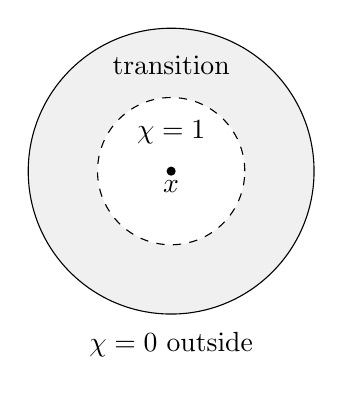
\begin{tikzpicture}[scale=1.1]
\fill[gray!12] (0,0) circle (1.65);
\fill[white] (0,0) circle (.85);
\draw (0,0) circle (1.65);
\draw[dashed] (0,0) circle (.85);
\fill (0,0) circle (1.5pt) node[below] {\(x\)};
\node at (0,.45) {\(\chi=1\)};
\node at (0,1.22) {transition};
\node at (0,-2) {\(\chi=0\) outside};
\end{tikzpicture}
\column{.53\textwidth}
Near \(x\): \(a\log|z|\) is psh.
\medskip
\par Outside the support: no change.
\medskip
\par On the annulus: derivatives of \(\chi\) may contribute negative curvature, but they are bounded.
\end{columns}
\end{frame}

\begin{frame}{A high power pays for the annulus}
For constants \(c>0,C_0,C_a\ge0\),
\[
i\Theta_L\ge c\omega,\quad
i\Theta_{K^{-1}}\ge-C_0\omega,\quad
2i\partial\db\psi_x\ge-C_a\omega.
\]
For \(h=h_L^N h_{K^{-1}}e^{-2\psi_x}\),
\[
i\Theta_h\ge(Nc-C_0-C_a)\omega.
\]
Choose \(N\) so the right side is strictly positive.
\end{frame}

\begin{frame}{First application: no base points}
Choose \(a=n\).
Our radial calculation gives
\[
\cI_h=\mathfrak m_x.
\]
Nadel gives
\[
H^1(X,L^N\otimes\mathfrak m_x)=0.
\]
Therefore \(H^0(X,L^N)\twoheadrightarrow (L^N)_x\).
\par Some global section is nonzero at \(x\).
\end{frame}

\begin{frame}{Second application: separate two points}
For distinct \(x,y\), use the sum of two logarithmic weights:
\[
\psi=\psi_x+\psi_y,\qquad a=n.
\]
Near \(x\), the weight \(\psi_y\) is smooth; similarly near \(y\).
Thus
\[
\cI_h=\mathfrak m_x\cap\mathfrak m_y.
\]
Nadel makes the evaluation map onto:
\[
H^0(X,L^N)\twoheadrightarrow (L^N)_x\oplus(L^N)_y.
\]
\end{frame}

\begin{frame}{Why this gives distinct projective points}
After choosing fibre coordinates, prescribe
\[
s(x)=1,\ s(y)=0,
\qquad
t(x)=0,\ t(y)=1.
\]
The evaluation functionals at \(x\) and \(y\) cannot be proportional.
\medskip
\par Hence
\[
\Phi_N(x)\ne\Phi_N(y).
\]
\end{frame}

\begin{frame}{Third application: prescribe the linear terms}
Choose \(a=n+1\) at \(x\).
Then
\[
\cI_h=\mathfrak m_x^2.
\]
Nadel gives surjectivity onto first jets:
\[
H^0(X,L^N)\twoheadrightarrow
H^0\bigl(X,L^N\otimes\cO_X/\mathfrak m_x^2\bigr).
\]
We can prescribe a section's value and all its first derivatives at \(x\).
\end{frame}

\begin{frame}{Why jets make the map an immersion}
In a local frame, choose sections with
\[
s_0=1+O(|z|^2),\qquad
s_j=z_j+O(|z|^2),\quad 1\le j\le n.
\]
On the chart \(s_0\ne0\), projective coordinates include \(s_j/s_0\).
\[
d\left(\frac{s_j}{s_0}\right)_x=dz_j.
\]
These span \(T_x^*X\), so \(d\Phi_N\) is injective.
\end{frame}

\begin{frame}{Why point separation alone is insufficient}
\begin{columns}[c]
\column{.47\textwidth}
\centering
\begin{tikzpicture}[scale=1.2]
\draw[->] (-.2,0)--(2,0) node[right] {\(x\)};
\draw[->] (0,-1.7)--(0,1.7) node[above] {\(y\)};
\draw[thick,domain=-1.1:1.1,samples=80,smooth,variable=\t] plot ({\t*\t},{\t*\t*\t});
\fill (0,0) circle (1.5pt);
\end{tikzpicture}
\column{.51\textwidth}
The cusp parametrization
\[
t\longmapsto(t^2,t^3)
\]
is injective, but its derivative vanishes at \(0\).
\medskip
\par First-jet separation rules out this failure.
\end{columns}
\src{Real slice of the complex cusp. Failure of immersion need not always produce a cusp.}
\end{frame}

\begin{frame}{One exponent must work for every point}
Choose finitely many coordinate charts with smaller charts covering \(X\).
Use cutoffs of a fixed radius around centres in each smaller chart.
\medskip
\par Their annular curvature losses have a uniform bound.
The sum of two point weights has at most twice that loss.
\medskip
\par Their supports may overlap: the singularities are still only at \(x\) and \(y\).
This avoids a bound that degenerates as \(y\to x\).
\end{frame}

\begin{frame}{Finish the embedding argument}
Choose one \(N\) dominating the uniform losses for
\[
\mathfrak m_x,\qquad
\mathfrak m_x\cap\mathfrak m_y,\qquad
\mathfrak m_x^2.
\]
The map \(\Phi_N\) is defined everywhere, injective, and an immersion.
\medskip
\par Since \(X\) is compact, \(\Phi_N\) is a homeomorphism onto its image.
Together with immersion, this makes it a holomorphic embedding.
\end{frame}

\begin{frame}{The converse takes one line}
If \(X\hookrightarrow\Pj^M\), restrict \(\cO_{\Pj^M}(1)\) with its Fubini--Study metric.
\[
i\Theta_{\cO(1)|_X}>0.
\]
More generally, if \(L^N\) defines an embedding, take the \(N\)-th root of its pulled-back metric.
\[
i\Theta_L=\frac1N\,i\Theta_{L^N}>0.
\]
Thus ampleness and positive curvature agree on a compact complex manifold.
\end{frame}

\begin{frame}{A historical pause: Kodaira}
Kodaira received the Fields Medal in 1954, becoming the first Japanese recipient.
\medskip
\par The IAS account highlights his work on harmonic analysis and the vanishing theorem.
\medskip
\par Our proof follows that analytic route all the way to a projective embedding:
\[
\text{curvature}\longrightarrow\text{cohomology}
\longrightarrow\text{sections}\longrightarrow\text{geometry}.
\]
\src{Institute for Advanced Study, scholar profile: Kunihiko Kodaira.}
\end{frame}

\begin{frame}{Now weaken positivity}
Kodaira vanishing assumes a smooth metric with strictly positive curvature.
\medskip
\par We now assume that \(L\) is only \emph{nef and big}, on a smooth projective variety.
\medskip
\par We will construct a strictly positive \emph{singular} metric with
\[
\cI_h=\cO_X.
\]
Nadel will then give ordinary cohomology vanishing.
\end{frame}

\begin{frame}{Intersection numbers in dimension (n)}
For line bundles \(L_1,\ldots,L_n\),
\[
L_1\cdots L_n
=\int_X c_1(L_1)\smile\cdots\smile c_1(L_n).
\]
For a curve \(C\subset X\),
\[
L\cdot C=\deg(L|_C)
\]
(with pullback to the normalization if needed).
\par On a surface this gives a bilinear pairing of divisor classes.
In higher dimension, a top intersection needs \(n\) divisor classes.
\end{frame}

\begin{frame}{Nef}
\[
\boxed{L\text{ is nef if }L\cdot C\ge0
\text{ for every irreducible curve }C\subset X.}
\]
On a projective variety, nef classes form the closure of the ample cone.
\medskip
\par We use the consequence:
\[
L\text{ nef},\ A\text{ ample}
\quad\Longrightarrow\quad L^m\otimes A\text{ ample},\ m\ge0.
\]
This does not assert that \(L\) has a smooth semipositive metric.
\end{frame}

\begin{frame}{Big}
\[
\boxed{L\text{ is big if }
\limsup_{m\to\infty}\frac{h^0(X,L^m)}{m^n}>0.}
\]
There are at least \(c\,m^n\) independent sections for arbitrarily large \(m\).
\medskip
\par The growth has the same order as for an ample bundle.
Bigness alone says nothing about positivity on each individual curve.
\end{frame}

\begin{frame}{A nef and big bundle need not be ample}
Let \(\pi:X=\operatorname{Bl}_p\Pj^2\to\Pj^2\) and \(L=\pi^*\cO(1)\).
\begin{center}
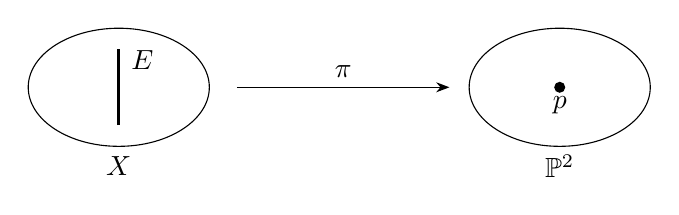
\begin{tikzpicture}[>=Stealth]
\draw (-3.4,0) ellipse (1.15 and .75);
\draw[very thick] (-3.4,-.48)--(-3.4,.48);
\node at (-3.1,.35) {\(E\)};
\node at (-3.4,-1) {\(X\)};
\draw[->] (-1.9,0)--(.8,0) node[midway,above] {\(\pi\)};
\draw (2.2,0) ellipse (1.15 and .75);
\fill (2.2,0) circle (2pt) node[below] {\(p\)};
\node at (2.2,-1) {\(\Pj^2\)};
\end{tikzpicture}
\end{center}
\[
L\cdot E=0,\qquad L^2=1,\qquad
h^0(X,L^m)=\binom{m+2}{2}.
\]
It is nef and big, but it contracts \(E\). The picture is schematic.
\end{frame}

\begin{frame}{Kawamata--Viehweg vanishing}
Let \(X\) be a smooth projective complex variety and \(L\) nef and big.
Then
\[
\boxed{H^q(X,K_X\otimes L)=0,\qquad q>0.}
\]
\medskip
\textbf{Kawamata--Viehweg:} obtain vanishing under the weaker positivity assumptions \textquotedblleft nef and big.\textquotedblright
\par We prove the line-bundle version.
\end{frame}

\begin{frame}{The metric we are looking for}
We want to write a power of \(L\) as
\[
L^N=(\text{ample bundle})\otimes\cO_X(D),
\qquad D\ge0.
\]
The ample factor supplies positive smooth curvature.
The divisor supplies a positive current.
\medskip
\par Taking an \(N\)-th root weakens the singularity on \(L\).
\end{frame}

\begin{frame}{Bigness produces an ample part}
Fix a smooth very ample divisor \(A\).
We claim that for some \(d>0\),
\[
\boxed{L^d\simeq\cO_X(A+D),\qquad D\ge0.}
\]
Equivalently, \(L^d\otimes\cO_X(-A)\) has a nonzero section.
\medskip
\par This is the form of Kodaira's lemma we need.
\end{frame}

\begin{frame}{Use the restriction sequence}
\[
0\longrightarrow L^m(-A)
\longrightarrow L^m
\longrightarrow L^m|_A
\longrightarrow0.
\]
Consequently
\[
h^0(X,L^m(-A))
\ge h^0(X,L^m)-h^0(A,L^m|_A).
\]
The first term grows like \(m^n\) along a subsequence.
The second is \(O(m^{n-1})\).
\end{frame}

\begin{frame}{Why the restriction has smaller growth}
On a projective variety \(Y\) of dimension \(r\), any fixed line bundle \(E\) satisfies
\[
h^0(Y,E^m)=O(m^r).
\]
Choose an effective ample \(H\) so \(E\otimes H\) is ample.
Multiplication by a section of \(H^m\) injects
\[
H^0(Y,E^m)\hookrightarrow H^0(Y,(E\otimes H)^m).
\]
Serre vanishing and the Hilbert polynomial bound the right side by \(O(m^r)\).
\par Apply this on \(Y=A\), \(r=n-1\).
\end{frame}

\begin{frame}{The dimension count, pictured}
\begin{center}
\begin{tikzpicture}[x=1cm,y=.65cm,>=Stealth]
\draw[->] (0,0)--(8,0) node[right] {\(m\)};
\draw[->] (0,0)--(0,4.7) node[above] {sections};
\draw[thick,domain=0:6.8,samples=60] plot (\x,{.09*\x*\x});
\draw[dashed,domain=0:7,samples=2] plot (\x,{.35*\x});
\node at (6,4.5) {\(c\,m^n\)};
\node at (6.1,1.3) {\(C\,m^{n-1}\)};
\end{tikzpicture}
\end{center}
Schematic growth comparison; bigness gives the lower bound along a subsequence.
\par For a sufficiently large such \(d\), \(h^0(X,L^d(-A))>0\).
\end{frame}

\begin{frame}{Now use nefness}
Keep the effective divisor \(D\) fixed.
For any \(N>d\),
\[
L^N=
\underbrace{L^{N-d}\otimes\cO_X(A)}_{M_N}
\otimes\cO_X(D).
\]
Since \(L\) is nef and \(\cO_X(A)\) is ample, \(M_N\) is ample.
\medskip
\par Choose a smooth positive metric \(h_N\) on \(M_N\).
\end{frame}

\begin{frame}{The divisor metric}
Let \(s_D\) be the canonical section of \(\cO_X(D)\).
Define its singular metric by
\[
|s_D|_{h_D}=1\quad\text{off }D.
\]
If \(s_D=f_De\), then
\[
|e|_{h_D}^2=|f_D|^{-2}.
\]
Poincaré--Lelong gives
\[
\boxed{i\Theta_{h_D}=2\pi[D]\ge0.}
\]
\end{frame}

\begin{frame}{Take an (N)-th root}
The product \(h_Nh_D\) is a metric on \(L^N\).
Thus
\[
h=(h_Nh_D)^{1/N}
\]
is a singular metric on \(L\), with
\[
i\Theta_h=\frac1N i\Theta_{h_N}+\frac{2\pi}{N}[D]
\ge\varepsilon_N\omega,\qquad \varepsilon_N>0.
\]
We only need positivity for this chosen \(N\), not a lower bound uniform in \(N\).
\end{frame}

\begin{frame}{How singular is the resulting metric?}
In a local frame,
\[
|e|_h^2=(\text{smooth positive factor})\,|f_D|^{-2/N}.
\]
The divisor \(D\) has stayed fixed while \(N\) increases.
\medskip
\par It remains to show
\[
|f_D|^{-2/N}\in L^1_{\mathrm{loc}}
\]
for sufficiently large \(N\).
\end{frame}

\begin{frame}{First test: a divisor with normal crossings}
Suppose locally
\[
f_D=z_1^{a_1}\cdots z_r^{a_r}.
\]
Then
\[
|f_D|^{-2/N}=\prod_{j=1}^r|z_j|^{-2a_j/N}.
\]
In each complex variable, the radial integral is
\[
\int_0^\delta r^{\,1-2a_j/N}\,dr<\infty
\quad\Longleftrightarrow\quad N>a_j.
\]
A sufficiently small exponent makes the singularity integrable.
\end{frame}

\begin{frame}{What if the divisor is singular?}
\textbf{Local integrability lemma.}
For every nonzero holomorphic \(f\), there is \(c>0\) such that
\[
|f|^{-2c}\in L^1_{\mathrm{loc}}.
\]
One proof uses Weierstrass preparation and integration in one variable.
\medskip
\par On compact \(X\), finitely many neighbourhoods give a common small exponent for the fixed divisor \(D\).
\par Choose \(1/N\) smaller than this exponent.
\end{frame}

\begin{frame}{A one-variable explanation of the lemma}
Weierstrass preparation gives, up to a bounded nonzero factor,
\[
f(z',w)=\prod_{j=1}^k(w-\alpha_j(z')).
\]
For each fixed \(z'\), Hölder gives
\[
\int\prod_{j=1}^k|w-\alpha_j|^{-2c}\,dA(w)
\le\prod_{j=1}^k
\left(\int|w-\alpha_j|^{-2ck}\,dA(w)\right)^{1/k}.
\]
These integrals are uniformly bounded when \(ck<1\).
Integrate over \(z'\) using Fubini.
\end{frame}

\begin{frame}{The multiplier ideal is now trivial}
The local weight itself is integrable, so
\[
1\in\cI_h.
\]
An ideal containing \(1\) is the whole ring.
Therefore
\[
\boxed{\cI_h=\cO_X.}
\]
We have made the singularity mild enough that no holomorphic germ is excluded.
\end{frame}

\begin{frame}{Finish Kawamata--Viehweg}
Our metric on \(L\) satisfies
\[
i\Theta_h\ge\varepsilon_N\omega,\qquad \cI_h=\cO_X.
\]
Nadel gives
\[
H^q(X,K_X\otimes L\otimes\cI_h)=0.
\]
Thus
\[
\boxed{H^q(X,K_X\otimes L)=0,\qquad q>0.}
\]
\end{frame}

\begin{frame}{What each hypothesis did}
\begin{enumerate}
\setlength{\itemsep}{10pt}
\item \textbf{Big:} obtain \(L^d=\cO_X(A+D)\), with \(A\) ample and \(D\) effective.
\item \textbf{Nef:} keep \(L^{N-d}\otimes\cO_X(A)\) ample as \(N\) grows.
\item \textbf{Large \(N\):} make the fixed divisor's singularity integrable.
\item \textbf{Nadel:} convert that metric into cohomology vanishing.
\end{enumerate}
\end{frame}

\begin{frame}{Historical order versus proof order}
Kawamata and Viehweg published their vanishing results in 1982.
Nadel's paper appeared in 1990.
\medskip
\par We have proved the older result using the later analytic theorem.
\medskip
\par This route makes both applications depend on a single question:
\[
\text{Which multiplier ideal does our metric produce?}
\]
\src{Y. Kawamata, \emph{Math. Ann.} 261 (1982), 43--46; E. Viehweg, \emph{J. reine angew. Math.} 335 (1982), 1--8; A. M. Nadel (1990).}
\end{frame}

\begin{frame}{Reading and proof boundaries}
\small
M. Verbitsky, \emph{Kähler geometry}, 2025 source for lecture 24 (Daniel): Kodaira embedding and Kawamata--Viehweg.
\medskip
\par Analytic input from lecture 23 (Daniel): Nadel vanishing.
\medskip
\par Projective inputs used here: nef plus ample is ample; Bertini; Serre vanishing and the Hilbert polynomial.
\medskip
\par The accompanying notes record sources, the uniform-cutoff argument, and the exact scope of the draft.
\end{frame}
\end{document}
